\chapter{Modelli e Funzionamento}\label{cap:modefunz}
\section{Blazor Server}\label{sez:bserver}
Il primo dei modelli ufficialmente rilasciati e per il quale si pu\`o ricevere supporto in produzione da settembre 2019\cite{blazorServerRelease}, \`e Blazor Server.

Un'applicazione Blazor Server ospita i componenti Blazor lato Server e gestisce le interazioni dell'utente con la UI attraverso una connessione in tempo reale sfruttando SignalR, come visibile nella figura \ref{fig:BlazorServer}.

SignalR \`e una libreria di software open-source sviluppata da Microsoft, che facilita l'interazione tra Client e Server, specialmente quando si necessita di mandare messaggi dal server ad uno o pi\`u client con un'alta frequenza~\cite{signalR}.
In particolare SignalR mette a disposizione delle API che permettono al codice che viene eseguito sul server di mandare messaggi real-time ad uno o pi\`u client connessi contemporaneamente, e questa libreria viene sfruttata dal modello Blazor Server per trasmettere a ciascun Client connesso, quali modifiche devono essere applicate al Document Object Model(da qui in poi abbreviato in DOM) perch\`e la UI di ciascun Client rispetti sempre la UI che il server mantiene in memoria.

\begin{figure}[H]
	\centerline{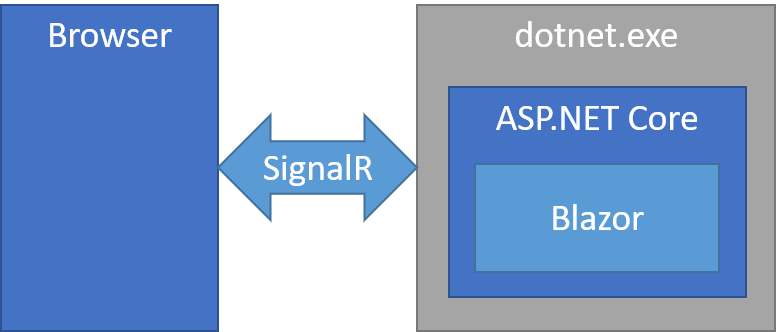
\includegraphics[scale=0.6]{figure/blazor-server.png}}
	\caption{Blazor Server}
	\label{fig:BlazorServer}
\end{figure}

Ci\`o significa che quando un utente scatena un evento, questo viene inviato attraverso la real time connection al server, dove il rispettivo componente di competenza gestisce l'evento.
Quando l'evento \`e stato gestito, Blazor compara l'output appena generato con quello precedente all'evento, e manda quindi le sole differenze al browser del client, per poi applicarle al DOM.\cite{blazorModelsScenarios}

Blazor Server perci\`o necessita di una connessione stabile e a bassa latenza per funzionare al meglio, e gli scenari offline non sono supportati.
Ci\`o significa anche che la posizione del server sul quale \`e ospitata l'applicazione non pu\`o essere troppo distante dal client che si sta connettendo per garantire un funzionamento senza lag.

Questo modello \`e particolarmente indicato quando si vuole delegare il costo computazionale al server e non ai client che ci si connettono, dato che ci\`o che il client deve computare \`e il solo codice statico scaricato inizialmente, e le differenze di volta in volta ricevute dal server, dove avviene invece la gestione di ogni evento e il calcolo delle differenze tra ci\`o che viene visualizzato prima di un evento e ci\`o che deve cambiare nella User-Interface del client dopo la sua gestione.
Ci\`o rende molto veloce ed efficiente il download iniziale e l'avvio dell'applicazione per gli utenti, il che lo rende il modello perfetto per funzionare su apparecchi a basso costo, che tuttavia devono sempre essere connessi ad internet.

\subsection{BlazorPong }\label{sez:bpong}
Un esempio di applicazione scritta con questo modello, \`e BlazorPong, appositamente implementata per questo lavoro di tesi e la cui demo \`e disponibile sul relativo repository in GitHub\cite{blazorPong}.

\begin{figure}[H]
	\centerline{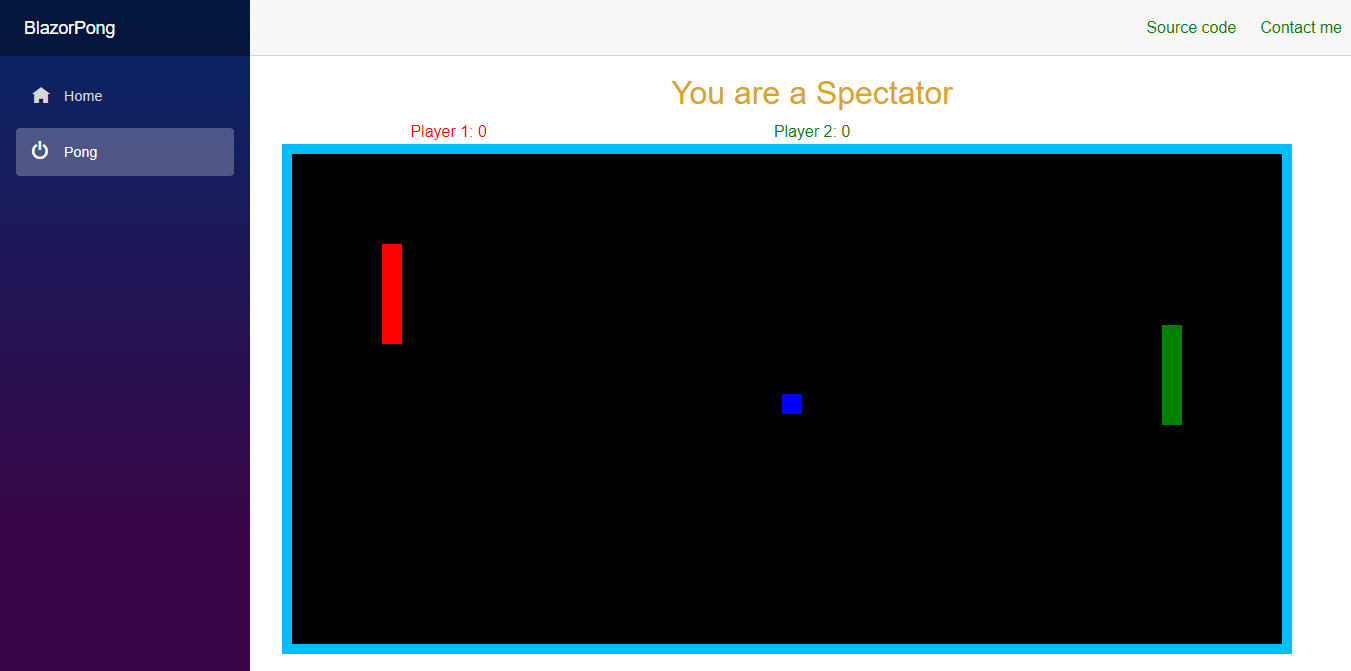
\includegraphics[scale=0.3]{figure/BlazorPong.PNG}}
	\caption{BlazorPong}
	\label{fig:BlazorPong}
\end{figure}

Questa applicazione, visibile nella figura \ref{fig:BlazorPong} permette a due giocatori che si collegano al sito contemporaneamente di giocare, e ai successivi utenti che si collegano di visionare la partita in corso come spettatori in tempo reale.
In questa applicazione \`e stato utilizzato il modello Blazor Server side per vari motivi:
\begin{enumerate}
	\item Il service worker che si occupa di aggiornare la posizione della pallina su tutti i client connessi, deve essere eseguito in un unico thread utilizzato per tutti i client connessi al server, ad ognuno dei quali invece devono arrivare gli aggiornamenti.
	\item Il calcolo delle differenze da applicare a ciascun DOM di ciascun utente connesso, per quanto avvenga continuamente(60 fps circa), conviene avvenga direttamente lato server poich\'e l'applicazione \`e molto semplice e infatti anche un host di livello gratuito come quello che si \`e scelto di utilizzare riesce a far giocare senza problemi due persone con diversi spettatori(i test che sono stati fatti sono tutti stati eseguiti dall'interno dell'europa, poich\'e il server utilizzato si trova in Francia).
	\item Essendo la gestione degli eventi server side, il gioco pu\`o essere visualizzato in modalit\`a spettatore senza problemi anche su cellulari non performanti.	
\end{enumerate}

Il funzionamento \`e piuttosto semplice: una volta che l'applicazione \`e stata avviata e che ciascun player si \`e connesso al sito ed ha cliccato play, quindi quando entrambi gli utenti sono pronti a giocare, inizia la partita.
Lato server viene gestito lo spostamento costante della pallina ed eventuali collisioni con muri verticali, orizzontali o con il blocco di uno dei player.
Rispettivamente gli eventi gestiti comunque dall'unico background worker condiviso che \`e eseguito sul Server, sono quindi:
\begin{enumerate}
	\item Collisione con un muro verticale con conseguente punto per il player che si trova dal lato opposto di quello in cui avviene la collisione;
	\item Collisione con un muro orizzontale con conseguente inversione della velocit\`a di spostamento della pallina sull'asse y;
	\item Collisione con uno dei blocchi dei giocatori con conseguente inversione della velocit\`a di spostamento della pallina sugli assi x ed y;
	\item L'arrivo a 3 punti di uno dei due giocatori o la disconnessione di uno dei due, gestito con l'invio di un messaggio di fine partita contenente il player vincitore a tutti gli utenti connessi.
\end{enumerate}

Ci\`o che invece avviene grazie all'utente, \`e lo spostamento del proprio player attraverso l'evento di drag del proprio blocco.
Ad ogni evento scatenato dall'utente, la connessione SignalR invia l'evento al server, che lo processa e restituisce a tutti gli utenti connessi(compreso quello che ha scatenato l'evento) la differenza di CSS necessaria a far combaciare l'immagine visualizzata con la nuova posizione reale del blocco del player che si \`e mosso.

\pagebreak

\section{Blazor WebAssembly}\label{sez:bwa}
Blazor WebAssembly \`e un modello attualmente in anteprima, e sar\`a ufficialmente rilasciato verso maggio del 2020.

In questo modello il codice della SPA viene scaricato ed eseguito nel browser del client che si collega alla SPA, come solitamente avviene quando si utilizza un framework moderno per UI come i gi\`a citati Angular, React e Vue.

\begin{figure}[H]
	\centerline{\includegraphics[scale=0.6]{figure/blazor-WebAssembly.png}}
	\caption{Blazor WebAssembly}
	\label{fig:BlazorWebAssembly}
\end{figure}

Vengono quindi scaricati dal client l'applicazione Blazor, le sue dipendenze, ed il runtime del .NET scelto come target per l'applicazione.
L'applicazione viene quindi eseguita direttamente nel thread della UI del Browser utilizzato, come visibile nella figura \ref{fig:BlazorWebAssembly}.

L'ambito di esecuzione \`e la stessa sandbox di qualsiasi altra applicazione scritta con javascript, ossia il browser che si sta utilizzando.
Ci\`o \`e importante perch\`e implica(ed \`e cos\'i) che una web app scritta utilizzando Blazor non pu\`o fare niente di pi\`u o di meno di una web app standard.
Ogni update alla UI e la relativa gestione, avvengono utilizzando lo stesso processo nel browser.
Per questo modello, blazor.WebAssembly.js \`e il nome dello script Javascript che si occupa di scaricare il .NET runtime compilato in WebAssembly, l'applicazione e le sue dipendenze, come anche dell'inizializzazione dell'applicazione.

\subsection{CLR e WebAssembly}\label{sez:webAssembly}
In particolare il nome Blazor WebAssembly per questo modello \`e stato scelto perch\`e nel browser di ciascun client che utilizza un'applicazione di questo tipo, viene scaricato ed utilizzato il file "mono.wasm".
Questo file contiene il CLR(Common Language Runtime) di Mono, una delle implementazioni del .NET Standard, compilato in WebAssembly.
Il runtime \`e necessario per poter eseguire i file compilati dell'applicazione e i pacchetti sulla quale si basa, che hanno estensione .dll e come target uno dei framework che implementano il .NET Standard(nel caso di Blazor, .NET Core), come visibile nella figura \ref{fig:CLR}.

\begin{figure}[H]
	\centerline{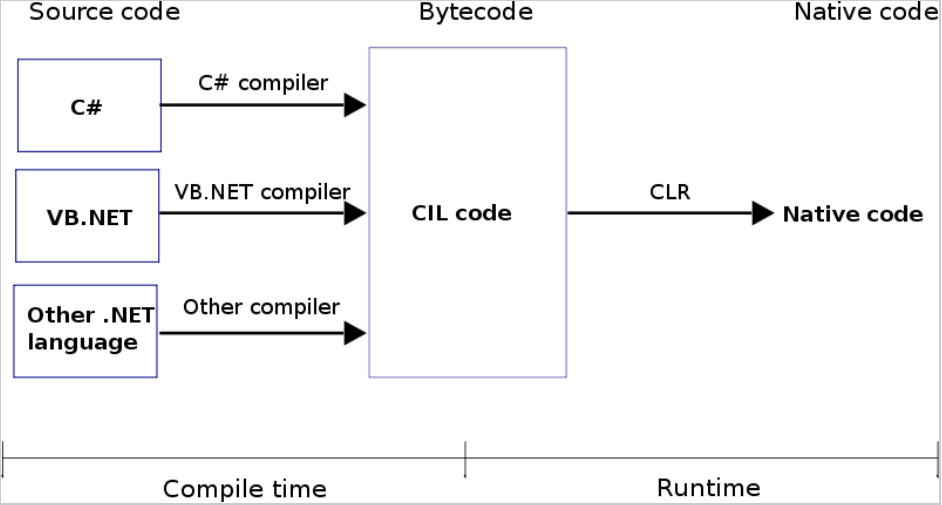
\includegraphics[scale=0.5]{figure/CLR.PNG}}
	\caption{Utilizzo del CLR}
	\label{fig:CLR}
\end{figure}

Il WebAssembly(da qui in poi abbreviato in WASM) \`e un formato per istruzioni binarie creato per essere il target della compilazione di linguaggi ad alto livello come C, C++, Rust\cite{webAssemblyOfficialWebsite}.
L'estensione .wasm \`e quella che \`e stata scelta per i file WASM.
Il progetto per la creazione di WASM \`e nato nel 2015, mentre dal 2017 i browser pi\`u diffusi al mondo come Chrome, Firefox, Edge e Safari si sono impegnati per svilupparlo ed adottarlo.\cite{webAssemblySupport}

\begin{figure}[H]
	\centerline{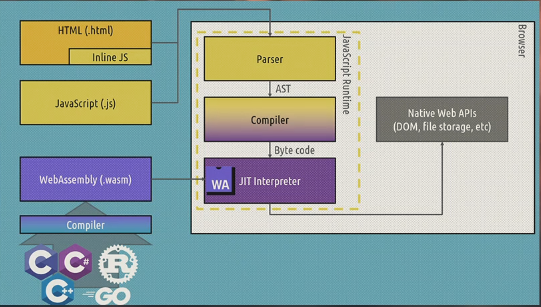
\includegraphics[scale=0.7]{figure/WasmVSJavascript.PNG}}
	\caption{Confronto tra WebAssembly e Javascript}
	\label{fig:WasmVSJavascript}
\end{figure}

Come si pu\`o vedere nella figura \ref{fig:WasmVSJavascript}, uno dei motivi per cui WASM \`e pi\`u veloce di Javascript \`e che non deve essere processato e compilato prima di poter essere interpretato, ma solamente scompattato ed eseguito e per questo motivo spesso viene definito il byte code per il web.

La compilazione avviene in modalit\`a AOT(Ahead of Time) e non pi\`u JIT(Just in Time), il che si traduce in un sensibile miglioramento delle prestazioni del codice dinamico.
Questa tecnologia \`e ci\`o che rende possibile il funzionamento di Blazor WebAssembly.

In questo modello quindi, come visibile dai Chrome Developer Tools, vengono scaricate le DLL dell'applicazione direttamente nel browser dell'utente.

\subsection{Blazor PWA}\label{sez:bpwa}
Il passaggio successivo per avvicinarsi al client allontanandosi dal modello server \`e poi Blazor PWA.

\`E cos\'i chiamato perch\`e in questo modello Blazor, permette di sviluppare l'interfaccia utente di una Progressive Web App.
Nella figura \ref{fig:WhatIsAPWA} viene riassunto cosa sia una Progressive Web App.

\begin{figure}[H]
	\centerline{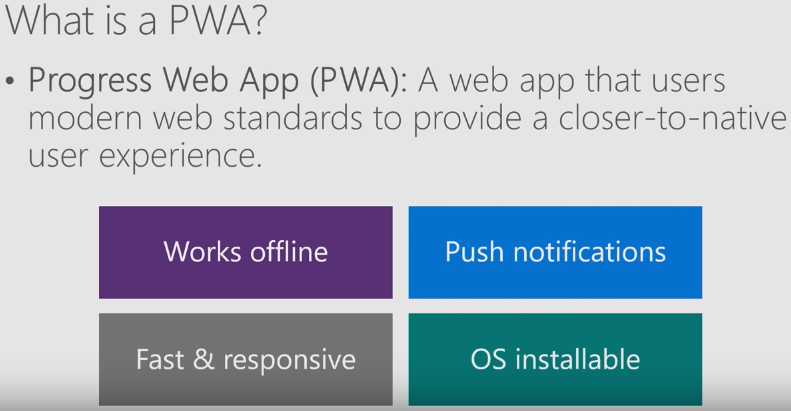
\includegraphics[scale=0.5]{figure/ProgressiveWebApp.png}}
	\caption{Progressive Web Apps}
	\label{fig:WhatIsAPWA}
\end{figure}

In particolare queste sono applicazioni web che hanno la capacit\`a di funzionare anche offline, e che spesso possono essere scaricate in modo persistente sulla macchina dell'utente che le esegue.
Offrono chiaramente una maggiore velocit\`a di esecuzione e la possibilit\`a di sfruttare alcune API native.
Ad esempio possono essere utilizzate quando la necessit\`a \`e quella di utilizzare le notifiche push native del sistema operativo che sta utilizzando il client(ad esempio Windows).

Al momento, per realizzare una PWA , bisogna partire dal modello Blazor WebAssembly aggiungendo un manifesto che descriva le capacit\`a dell'applicazione, i permessi richiesti e l'icona da utilizzare una volta installata, oltre chiaramente a dover implementare l'applicazione in modo che possa lavorare anche offline, basandosi su un service worker.\cite{blazorPWA}
\pagebreak

\section{Modelli in roadmap}
\subsection{Blazor Hybrid}\label{sez:bhybrid}
Questo modello di Blazor ed anche il successivo, servono a sviluppare applicazioni native.
Nel modello Hybrid, l'applicazione sviluppata non \`e quindi pi\`u considerabile una web app ma rimane ibrida perch\`e pur essendo un'applicazione con capacit\`a native, utilizza tecnologie web per effettuare il rendering della UI.

Esempi di Hybrid Apps possono essere applicazioni mobile native, che hanno accesso alle API esposte ad esempio da Android, ma che utilizzano delle WebViews per la gestione dell'interazione dell'utente con la UI.
Un altro esempio molto interessante sono le applicazioni, scritte in Blazor, che sfruttano Electron.

Electron \`e un framework open-source sviluppato e mantenuto da GitHub, precedentemente noto come Atom Shell.
In particolare Electron permette di sviluppare interfacce grafiche per desktop eseguibili su Windows, Linux e macOS utilizzando tecnologie web \cite{electronWiki}.
Electron combina il motore di rendering del browser Chromium ed il runtime Node.js, che vengono inclusi in ogni applicazione sviluppata utilizzando questo framework.
Utilizzando quindi il pacchetto Electron.NET, si pu\`o fare in modo di eseguire un'applicazione .NET Core nell'ambiente(browser e runtime) esposto da Electron, utilizzando Blazor in fase di sviluppo\cite{electronDotNet}.

In questo modo si pu\`o ottenere un'applicazione con capacit\`a native, che sia cross-platform, la cui interfaccia sia stata scritta utilizzando Blazor.
Nella figura \ref{fig:BlazorHybridApplication} si pu\`o vedere una Web Application compilata nativamente con Electron(con target Windows), e quindi eseguita come applicazione desktop:

\begin{figure}[H]
	\centerline{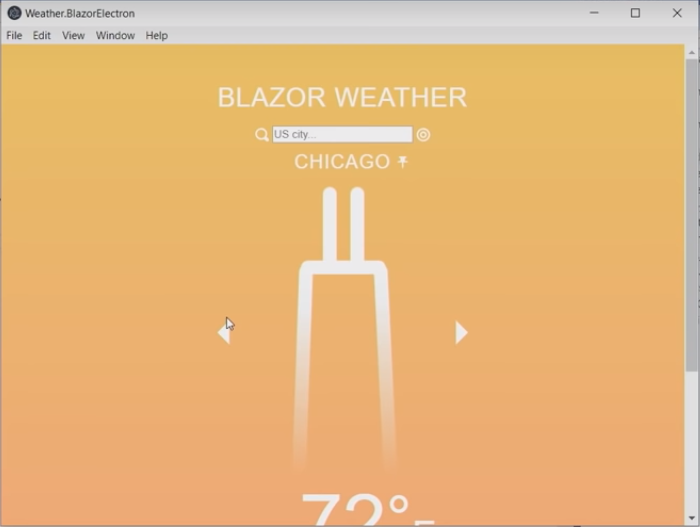
\includegraphics[scale=0.6]{figure/BlazorWeatherElectron.png}}
	\caption{Blazor Hybrid Application}
	\label{fig:BlazorHybridApplication}
\end{figure}

Il codice open source di questa applicazione, si pu\`o trovare al seguente link: https://github.com/danroth27/BlazorWeather/tree/master/BlazorWeather.Electron
\pagebreak

\subsection{Blazor Native}\label{sez:bnative}
Infine esiste il modello Native che \`e possibile grazie al fatto che Blazor \`e stato architettato per poter renderizzare controlli della UI che non siano obbligatoriamente strumenti web, e pu\`o quindi integrarsi con controlli nativi.
Il rendering layer \`e infatti intercambiabile, pur essendo quello di default dedicato all'HTML.

Un esempio di applicazione sviluppata utilizzando Blazor per il rendering di controlli nativi nella UI, si pu\`o vedere durante la presentazione di Steve Sanderson all'evento NDC Oslo di quest'anno, pur non essendo stato ancora rilasciato il codice di un esempio ufficiale.\cite{sandersonNDCBlutter}
In questa applicazione, si \`e scelto di sostituire il default rendering layer per utilizzarne uno personalizzato, utilizzando componenti di Flutter, il toolkit di Google per costruire interfacce utente native CrossPlatform.
Questo modello viene qui citato per completezza, ma al momento non \`e nemmeno presente nella documentazione ufficiale ed \`e solo stato citato da Daniel Roth durante la presentazione dei futuri modelli di Blazor lato client.\cite{blazorNative}

\section{Funzionamento}\label{sez:funzionamento}
Quando si scrive si utilizza un mix di HTML per lo scheletro, CSS per lo stile del documento e C\# preceduto dal relativo carattere di escape(@) per la parte dinamica del codice.
\begin{figure}[H]
	\centerline{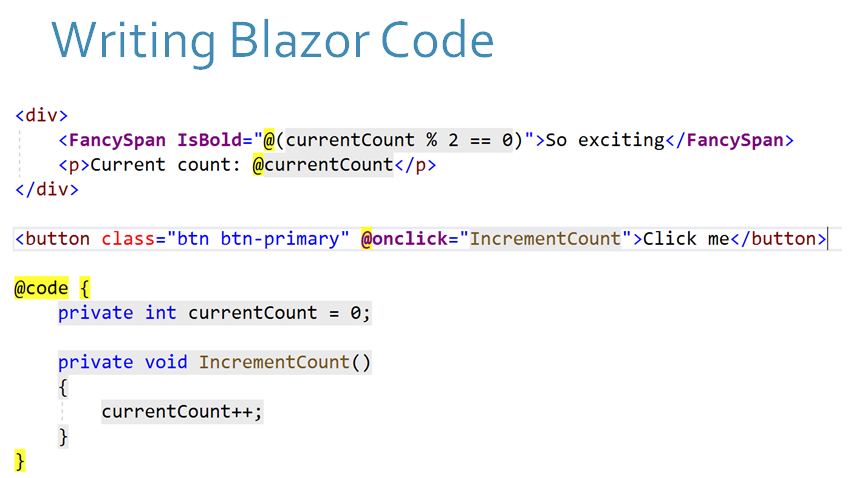
\includegraphics[scale=0.55]{figure/RazorFile.png}}
	\caption{File Razor\cite{ryanNowakNDCSydney}}
	\label{fig:razorFile}
\end{figure}
Si pu\`o scrivere utilizzando questa sintassi solamente nei file che hanno estensione ".razor", il cui esempio si pu\`o trovare in figura \ref{fig:razorFile}.
Quando l'applicazione viene compilata, i file .razor vengono utilizzati come input per generare dei file C\#(quindi con estensione .cs) equivalenti al codice che si \`e descritto.\cite{ryanNowakNDCSydney}
Un esempio di output di file razor compilato, generato a partire da quello in figura \ref{fig:razorFile} \`e visibile in figura \ref{fig:compiledRazorFile}.
\begin{figure}[H]
	\centerline{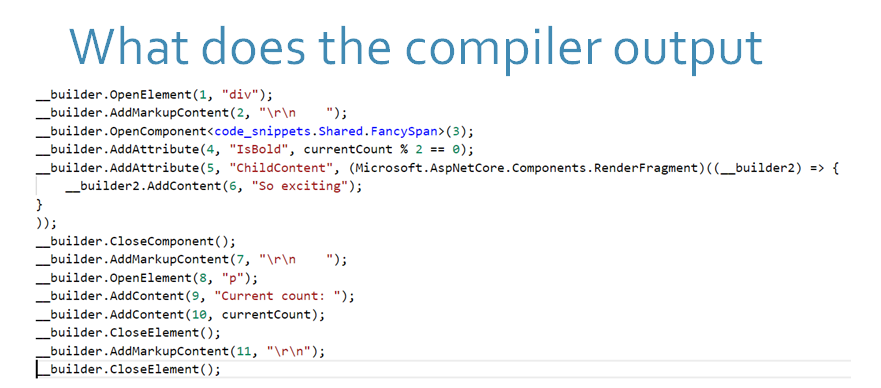
\includegraphics[scale=0.55]{figure/RazorFileCompiled.PNG}}
	\caption{Output\cite{ryanNowakNDCSydney}}
	\label{fig:compiledRazorFile}
\end{figure}

Saranno poi questi file ad essere effettivamente utilizzati da Roslyn(che \`e il nome del compilatore open-source del linguaggio C\#) e a finire nella DLL generata come output dal progetto nel quale si trova il file .razor di partenza.
Questo passaggio non \`e solo necessario per fare in modo che si possano generare le DLL compilate relative ai file di partenza, ma \`e anche il momento in cui viene ottimizzato ci\`o che ha scritto il developer per ogni parte relativa alla UI in ogni file .razor del progetto, riducendolo alle sole primitive di Blazor, che sono visibili nella figura \ref{fig:BlazorPrimitives}.

\begin{figure}[H]
	\centerline{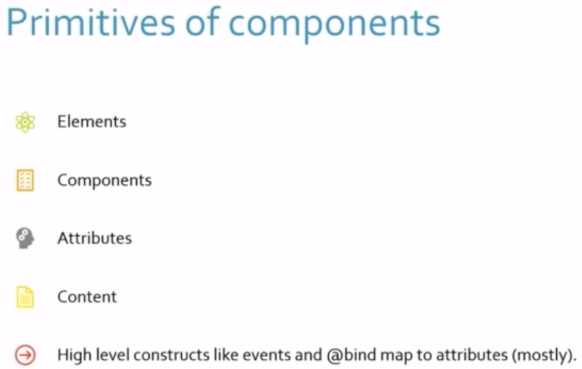
\includegraphics[scale=0.7]{figure/BlazorPrimitives.PNG}}
	\caption{Primitive di Blazor\cite{ryanNowakNDCSydney}}
	\label{fig:BlazorPrimitives}
\end{figure}

In ordine quindi possiamo descrivere le primitive:
\begin{enumerate}
	\item Un elemento \`e ad esempio l'elemento html "div";
	\item Un component \`e un altro componente(file .razor) che viene utilizzato nel file che si sta compilando;
	\item Un attributo \`e appunto un attributo di un elemento html, o un parametro passato in ingresso ad un component;
	\item Un contenuto \`e del testo, costante o basato su un parametro, inserito all'interno di un elemento html;
	\item L'ultima primitiva di un componente Blazor sono sostanzialmente gli eventi che vengono gestiti dal componente che si sta compilando e le direttive di bind che quindi collegano e mantengono sincronizzate due variabili.
\end{enumerate}

\pagebreak